% Provenance (never printed): see sources/outline_sources.md (Year 2: monsoons; El Niño--Southern
% Oscillation; the North Atlantic Oscillation; ocean--atmosphere coupling). Definitions after the
% IPCC AR6 glossary, the NOAA CPC ENSO FAQ and NAO pages, the NWS glossary and the IMD monsoon
% FAQ; indices from the CPC data files (data/derived/bachelor-2-{oni,oni-table,roni,nino34,nao});
% figures from figdata/bachelor-2/climvar.py; values of the examples, exercises and problem
% computed in the Book 4 scratch calculator calc/ch23.py.
\chapter{气候变率}\label{ch:b2:climate-variability}

2026年9月，赤道中太平洋的海表面温度平均为 \qty{29.27}{\celsius}，
通常的9月值为 \qty{26.71}{\celsius}；更东部的部分海域比往常高出
\qty{4}{\celsius} 以上，预报员认为，到年底该事件超过
自1950年以来每一次\omterm{def:b2:climate-variability:enso}{厄尔尼诺}的可能性在五分之四以上。此前的
纪录事件发生于1982年、1997年和2015年，使珊瑚白化死亡、热带森林起火，
并带来热浪；每当这样的暖水持续滞留，秘鲁凤尾鱼的渔获量便急剧下降。
热带太平洋的海洋与大气如每隔数年一次那样发生摆动，
这一摆动远远超出了太平洋。本
章介绍气候的这类摆动：\omterm{def:b2:climate-variability:monsoon}{季风}、\omterm{def:b2:climate-variability:enso}{厄尔尼诺}与\omterm{def:b2:climate-variability:enso}{拉尼娜}、
\omterm{def:b2:climate-variability:nao}{北大西洋涛动}，以及使海洋成为这些摆动“记忆”的原因。
% ledger: data:b4-nino34, cpc:edd-2026-10, thirumalai24:bjerknes, cheung26:peru

\begin{recall}
\textbf{来自中学分册}：天气与气候；温度距平；混合层，
温跃层和上升流；气候反馈。\textbf{来自本科一年级分册}：哈得来
环流圈、信风、热带辐合带及其季节性迁移、沃克
环流、沿岸上升流。\textbf{来自\cref{ch:b2:weather-systems}}：急流、
\omterm{def:b2:weather-systems:rossby}{罗斯贝波}、\omterm{def:b2:weather-systems:cyclones}{温带气旋}和阻塞。\textbf{来自物理学各册}：热容
及热力学第一定律。
\end{recall}

\section{变率及其度量}\label{sec:b2:climate-variability:measures}

天气逐日变化；气候作为天气的统计特征，即使气候系统之外没有任何变化，也会
从一个季节或一年到下一个季节或下一年而变化。其中一部分是噪声，但
变率的大部分有组织地构成若干反复出现的型态，各有其
空间分布、季节特征和时间尺度。

\begin{definition}[气候变率模态；气候指数；气候态]\label{def:b2:climate-variability:modes}
称\emph{气候变率模态}\index{气候变率模态}为一种反复出现的
气候系统自然变率型态，具有自身的空间型态、季节性和时间尺度，
由大气的动力学过程产生，或由海洋与大气的偶联引起。
称\emph{气候指数}\index{气候指数}为由气候变量构成、概括该型态状态的时间序列，
例如冰岛与亚速尔群岛之间的海平面气压差。
变量的\emph{气候态}\index{气候态}是其在参考时段内的平均值，
按每个日历月或每个季节分别计算；
标准参考时段为30年，目前为1991--2020年。
\end{definition}
% ledger: ipccgl:modes, ipccgl:index, wmo:normal-30yr

许多模态由气候系统内部的过程驱动，它们属于气候系统的
内部变率。由于它们以各自的时间尺度反复出现，它们是
超出天气预报范围的可预报性来源，时间尺度从数周到数十年。指数使这些模态
可以被度量。指数由距平计算得出，如中学分册所述，并
作平滑处理。
% ledger: ipccgl:modes

\begin{method}[从观测到指数]\label{met:b2:climate-variability:index}
\begin{enumerate}
  \item 计算\omterm{def:b2:climate-variability:modes}{气候态}：对每个日历月，求该变量在
        参考时段内的平均值。
  \item 减去\omterm{def:b2:climate-variability:modes}{气候态}：每个月的距平为该月数值减去该月的\omterm{def:b2:climate-variability:modes}{气候态}。
        季节循环随之消失，余下的即为变率。
  \item 对距平作滑动平均，即取以各月为中心的 $n$ 个连续值的
        平均，以去除短于所关注型态的波动。
  \item 若指数要与其他指数比较，则除以其标准差，
        使指数以标准差为单位标准化。
\end{enumerate}
\end{method}

\begin{example}[距平]\label{ex:b2:climate-variability:anomaly}
赤道中太平洋（北纬 \ang{5} 与南纬 \ang{5}，西经 \ang{170} 至
\ang{120} 之间）的平均海表面温度，2026年9月为 \qty{29.27}{\celsius}。
9月的\omterm{def:b2:climate-variability:modes}{气候态}为 \qty{26.71}{\celsius}，因此距平为 $29.27 - 26.71 = \qty{2.56}{\celsius}$。
1997年9月同一海域为 \qty{28.79}{\celsius}，而\omterm{def:b2:climate-variability:modes}{气候态}为 \qty{26.73}{\celsius}，
距平为 \qty{2.06}{\celsius}。两个\omterm{def:b2:climate-variability:modes}{气候态}略有差异，原因在于参考时段
每五年推进一次：海洋本身已经变暖。
% ledger: data:b4-nino34, cpc:oni-def
\end{example}

\section{季风}\label{sec:b2:climate-variability:monsoons}

\begin{definition}[季风]\label{def:b2:climate-variability:monsoon}
称\emph{季风}\index{季风}为一种热力驱动的风，由陆地与邻近海洋
的不同受热所引起，其风向随季节反转，并伴随
其所带来降水的季节性反转。
\end{definition}
% ledger: nws4:monsoon, ipccgl:monsoon

夏季阳光的热量在陆地上只停留在近地表的薄层中，而海洋
则将同样的热量经混合层向下混合（混合层深达数十米），升温要小得多。
陆地上空的空气增温更多，地面气压下降，湿润空气自海洋流入，上升、冷却并
降雨；高空空气则向海回流。冬季陆地是较冷的下垫面，环流
随之反转。综合来看，全球\omterm{def:b2:climate-variability:monsoon}{季风}构成一个统一的全球型态，主导着年循环
热带与副热带降水的年循环；其范围定义为当地夏季的平均降水
较冬季每天多出超过 \qty{2.5}{mm} 的地区。
% ledger: nws4:monsoon, ipccgl:monsoon

\begin{omfigure}
\centering
\begin{tikzpicture}[font=\scriptsize, >=Stealth]
\foreach \col/\title in {0/{a\enspace 夏季}, 7.2/{b\enspace 冬季}} {
  \begin{scope}[shift={(\col,0)}]
  \node[anchor=south west] at (0,3.0) {\textbf{\title}};
  \fill[ocBlue!18] (0,0) rectangle (3,0.35);
  \fill[brown!35] (3,0) -- (6.4,0) -- (6.4,0.5) -- (3,0.35) -- cycle;
  \node at (1.5,0.17) {海洋};
  \node at (4.7,0.2) {陆地};
  \end{scope}
}
% summer: low over the land, inflow from the sea, rising air and rain
\node[font=\small\bfseries, ocBlue] at (0.45,0.62) {H};
\node[font=\small\bfseries, ocRed] at (4.8,0.78) {L};
\node[ocRed, anchor=west] at (5.35,0.78) {热};
\draw[->, thick] (1.0,0.98) -- (4.2,1.02);
\node at (2.4,0.66) {湿润空气来自海洋};
\draw[->, thick] (4.8,1.15) -- (4.8,2.55);
\draw[->, thick] (4.45,2.8) -- (1.75,2.8);
\draw[->, thick] (1.4,2.6) -- (1.4,1.25);
\fill[black!15, draw=black!40] (4.0,1.9) .. controls (4.0,2.55) and (5.6,2.55) .. (5.6,1.9) -- cycle;
\foreach \x in {4.25,4.5,5.1,5.35} {\draw[ocBlue, dashed] (\x,1.85) -- (\x-0.1,1.2);}
\node[anchor=west] at (5.65,2.1) {降雨};
% winter: high over the land, dry outflow to the sea
\begin{scope}[shift={(7.2,0)}]
\node[font=\small\bfseries, ocRed] at (0.45,0.62) {L};
\node[font=\small\bfseries, ocBlue] at (4.8,0.78) {H};
\node[ocBlue, anchor=west] at (5.35,0.78) {冷};
\draw[->, thick] (4.2,1.02) -- (1.0,0.98);
\node at (2.4,0.66) {干燥空气来自陆地};
\draw[->, thick] (1.4,1.25) -- (1.4,2.6);
\draw[->, thick] (1.75,2.8) -- (4.45,2.8);
\draw[->, thick] (4.8,2.55) -- (4.8,1.15);
\end{scope}
\end{tikzpicture}
\par\smallskip{\small \omterm{def:b2:climate-variability:monsoon}{季风}作为陆海环流（示意剖面，不按比例）：
夏季陆地是较暖的下垫面，地面为低压，湿润空气流入，
自海洋而来，上升并降雨；冬季环流反转，陆地吹来的风干燥。}
\end{omfigure}
% ledger: nws4:monsoon, imd:heat-low

南亚与东南亚的\omterm{def:b2:climate-variability:monsoon}{季风}始于五月下旬或六月初，
向东北推进，并于九月下旬或十月初结束。\omterm{def:b2:climate-variability:monsoon}{季风}到来之前，阿拉伯海周围的陆地增温：
六月时，地表向上空输送约 \qty{160}{W/m^2} 的热量，覆盖
印度西北部干旱地区、巴基斯坦和中东，那里形成一个浅薄的热低压，
高度仅达约 \qty{1.5}{km}，雨量很少；热低压较弱时（如 1987 年的干旱年份），
意味着对海洋上湿润空气的拉力较弱。由此形成一条狭长的低压槽，即\omterm{def:b2:climate-variability:monsoon}{季风}槽，
延伸至孟加拉湾顶部；\omterm{def:b2:climate-variability:monsoon}{季风}槽的南北摆动带来季节中的活跃期与间歇期。
就印度全境而言，六月至九月的降雨量平均为
\qty{88}{cm}，标准差为 \qty{9}{cm}，约为 \qty{10}{\percent}：与长期平均值相差
在 \qty{10}{\percent} 以内的季节称为正常。在喀拉拉邦海岸，国家气象部门宣布\omterm{def:b2:climate-variability:monsoon}{季风}开始，依据的是
十四个站点的降雨量，
风以及卫星测得的向外红外辐射。此处平均降雨量
六月为 \qty{556}{mm}，七月为 \qty{659}{mm}。
% ledger: ipccgl:monsoon, imd:heat-low, imd:lpa, imd:onset

西非\omterm{def:b2:climate-variability:monsoon}{季风}自几内亚湾带来湿润的西南风，
五月至九月向北推进；其降雨在八月下旬和九月于北纬 \ang{12} 附近达到峰值，
十月起后撤。
% ledger: ipccgl:monsoon

\omterm{def:b2:climate-variability:monsoon}{季风}时间上规律性强，雨量却不稳定，其逐年波动
部分原因在于热带太平洋的变化。\omterm{def:b2:climate-variability:enso}{厄尔尼诺}年份往往使印度降雨不足：
1904 年、1972 年和 1987 年的干旱都伴随\omterm{def:b2:climate-variability:enso}{厄尔尼诺}出现。两者的关联并不确定：1997 年
一次强\omterm{def:b2:climate-variability:enso}{厄尔尼诺}与印度洋偶极子的正位相同时出现，该模态见下文，而印度
的\omterm{def:b2:climate-variability:monsoon}{季风}接近正常。
% ledger: narang24:enso-monsoon, ipccgl:other-modes

\section{厄尔尼诺与南方涛动}\label{sec:b2:climate-variability:enso}

本科一年级分册介绍过沃克环流：空气在温暖的西太平洋上升，
在高空向东流动，在较冷的东太平洋下沉，并随信风
向西返回。海洋中，信风把暖水推向西部，那里温跃层较深；
同时沿赤道把冷水向东部翻升，那里温跃层较浅。这种状态并不
固定。

\begin{definition}[厄尔尼诺–南方涛动；厄尔尼诺；拉尼娜；南方涛动]\label{def:b2:climate-variability:enso}
\emph{厄尔尼诺–南方涛动}\index{厄尔尼诺–南方涛动}（ENSO）
是热带太平洋的海洋–大气耦合模态，表现为相干的年际变化，
包括海表温度、对流降雨、地面气压以及沿赤道太平洋的环流，
其偏好的时间尺度为两至七年左右。\emph{厄尔尼诺}\index{厄尔尼诺}
是其暖相位，即赤道太平洋中部和中东部海表的增温；
\emph{拉尼娜}\index{拉尼娜}是其冷相位，即同一区域的
降温。\emph{南方涛动}\index{南方涛动}是其大气部分，
表现为热带太平洋东西两侧地面气压的跷跷板变化：厄尔尼诺期间
印度尼西亚和西太平洋上气压高于平均值，东太平洋上则低于平均值，
拉尼娜期间则相反。
\end{definition}
% ledger: cpc:enso-faq, cpc:enso-faq-so, ipccgl:enso

\omterm{def:b2:climate-variability:enso}{厄尔尼诺}期间，赤道上的信风减弱，在西部
低层风甚至可能吹西风；西部的暖水向东扩展，深对流
及其降雨随之东移，使印度尼西亚与澳大利亚北部更加干燥。海表
温度在东中部太平洋通常比平均值高 \qtyrange{1.5}{2.5}{\celsius}，
那里的温跃层位于 \qtyrange{150}{175}{m}，比平常更深。\omterm{def:b2:climate-variability:enso}{拉尼娜}期间，信风
在整个海盆增强，海表温度比平均值低 \qtyrange{1}{2}{\celsius}，
东部温跃层升至 \qtyrange{50}{100}{m}。沃克环流
在\omterm{def:b2:climate-variability:enso}{厄尔尼诺}期间减弱，在\omterm{def:b2:climate-variability:enso}{拉尼娜}期间增强。事件通常每三至
五年重现一次，间隔在两至七年之间变化；\omterm{def:b2:climate-variability:enso}{厄尔尼诺}通常持续九至
十二个月，\omterm{def:b2:climate-variability:enso}{拉尼娜}则持续一至三年。两者通常在三月至六月之间发展，
在十二月至次年四月达到峰值，于五月至七月减弱；影响最强的时段是
十二月至次年四月，即赤道海表最暖的时候。
% ledger: cpc:enso-faq-features, cpc:enso-faq-timing

\begin{omfigure}
\centering
\begin{tikzpicture}[font=\scriptsize, >=Stealth, x=1cm, y=0.8cm]
\foreach \row/\title/\tw/\te/\rx/\cwidth in {
    0/{a\enspace 中性}/1.15/0.35/1.6/1.0,
    -4.6/{b\enspace 厄尔尼诺}/0.95/0.85/5.6/1.4,
    -9.2/{c\enspace 拉尼娜}/1.3/0.18/1.0/0.8} {
  \begin{scope}[shift={(0,\row)}]
  \node[anchor=south west] at (0,2.55) {\textbf{\title}};
  % ocean: warm layer above the thermocline
  \fill[ocBlue!20] (0,-1.5) rectangle (11,0);
  \fill[omWarm!25] (0,0) -- (0,-\tw) .. controls (4,-\tw) and (7,-\te) .. (11,-\te) -- (11,0) -- cycle;
  \draw[thick, ocBlue!70!black] (0,-\tw) .. controls (4,-\tw) and (7,-\te) .. (11,-\te);
  \draw (0,0) -- (11,0);
  % convection and Walker cell
  \fill[black!15, draw=black!40] ({\rx-\cwidth/2},0.5) .. controls ({\rx-\cwidth/2},2.1) and ({\rx+\cwidth/2},2.1) .. ({\rx+\cwidth/2},0.5) -- cycle;
  \draw[->, thick] (\rx,0.55) -- (\rx,2.15);
  \draw[->, thick] ({\rx+0.4},2.3) -- (9.6,2.3);
  \draw[->, thick] (10.0,2.1) -- (10.0,0.5);
  \draw[->, thick] (9.6,0.3) -- ({\rx+0.7},0.3);
  \end{scope}
}
\node[anchor=west] at (2.3,1.4) {上升空气，降雨};
\node[anchor=east] at (9.9,1.4) {下沉空气};
\node at (6.0,0.55) {信风};
\node[anchor=west, ocBlue!70!black] at (7.6,-0.95) {温跃层};
\node[anchor=east] at (4.8,-4.6+1.4) {降雨东移};
\node at (8.2,-4.6+0.55) {较弱的信风};
\node at (6.0,-9.2+0.55) {较强的信风};
\node[ocBlue!70!black, align=center] at (9.6,-9.2-0.8) {冷水 \\位于表层附近};
\node[anchor=north west] at (0,-9.2-1.55) {西部（印度尼西亚）};
\node[anchor=north east] at (11,-9.2-1.55) {东部（南美洲）};
\end{tikzpicture}
\par\smallskip{\small 沿赤道的太平洋在 ENSO 三种位相中的状况
（示意，不按比例）：上方为沃克环流，下方为暖上层和
温跃层。\omterm{def:b2:climate-variability:enso}{厄尔尼诺}期间信风减弱，暖水与降雨向东扩展，
东部温跃层加深至 \qtyrange{150}{175}{m}；\omterm{def:b2:climate-variability:enso}{拉尼娜}期间信风
增强，东部温跃层升至 \qtyrange{50}{100}{m}。}
\end{omfigure}
% ledger: cpc:enso-faq-features, climategov:walker

这些名称出自不同的时代与不同的学科。南美洲海岸的渔民
注意到圣诞节前后近岸海水增温，扰乱了渔业，
便称之为\omterm{def:b2:climate-variability:enso}{厄尔尼诺}，意为“小男孩”。吉尔伯特·沃克爵士在大气中发现了\omterm{def:b2:climate-variability:enso}{南方涛动}，
但未将其与海洋联系起来。直到 20 世纪 60 年代末，雅各布·皮耶克尼斯等人才看出
两者是同一现象。“\omterm{def:b2:climate-variability:enso}{拉尼娜}”与“中性”等术语在 20 世纪 80 年代开始广为使用。
% ledger: climategov:enso-history, ipccgl:enso

\begin{history}[渔民的“小男孩”]
\begin{minipage}[t]{0.54\linewidth}\vspace{0pt}
秘鲁干旱的海岸附近，风沿岸将冷水向上推送，这些冷水富含
营养物质，养育着高产的渔业。当地渔民知道，每年圣诞节前后会出现一次增温，
此时鱼群变得稀少，他们便以“季节之子”为其命名。
秘鲁的凤尾鱼渔获量至今仍受 ENSO 影响：近期一项分析中，长时间的高温距平
使极低渔获量出现的可能性增至九倍以上，渔获量的中位数降幅
约为 \qty{60}{\percent}；1997--98 年的强\omterm{def:b2:climate-variability:enso}{厄尔尼诺}事件在记录中尤为突出。
\end{minipage}\hfill
\begin{minipage}[t]{0.42\linewidth}\vspace{0pt}
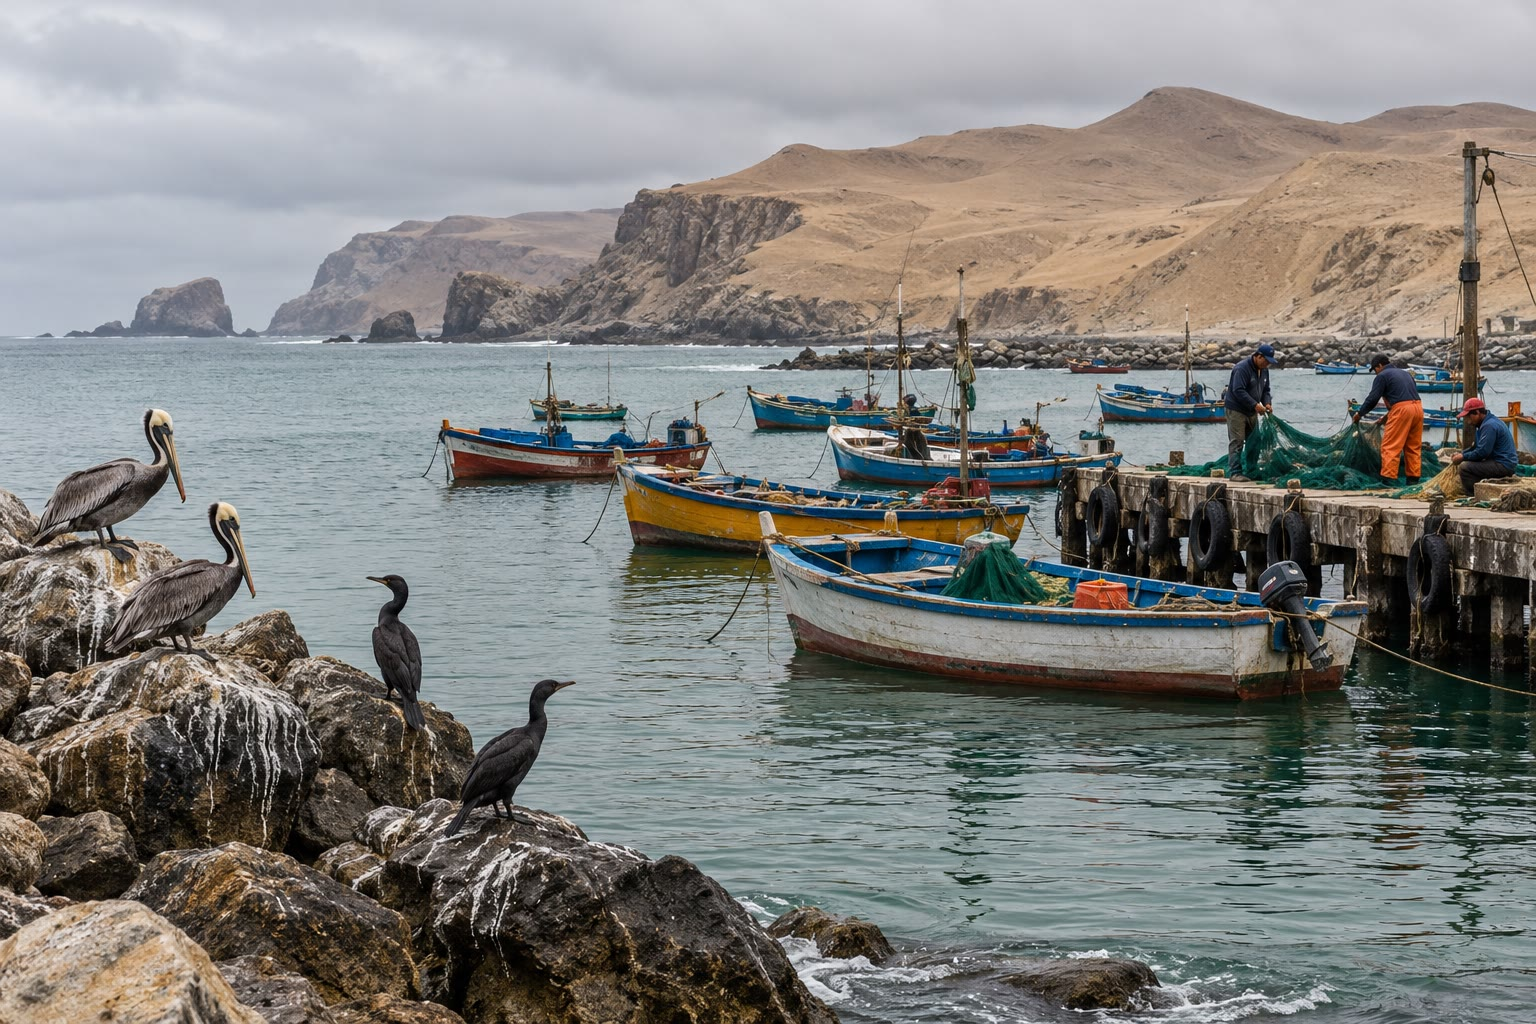
\includegraphics[width=\linewidth]{images/book4/ai/b2-fishing-harbour.jpg}

{\scriptsize 干旱海岸港口中的渔船，周围是冷的上升流海水
（AI 生成插图）。}
\end{minipage}
% ledger: climategov:enso-history, cheung26:peru, stewart:upwelling
\end{history}

系统为何会振荡？因为赤道太平洋的海洋与大气
相互加强彼此的距平。

\begin{definition}[皮耶克尼斯反馈]\label{def:b2:climate-variability:bjerknes}
称\emph{皮耶克尼斯反馈}\index{皮耶克尼斯反馈}为赤道太平洋的海表温度、风与
洋流之间的正反馈：东部增温会削弱东西向的温度与气压对比，
进而使信风减弱；
信风减弱使西部暖水向东扩展，东部上升的冷水减少，
东部因而进一步增温。同一循环也会放大降温。
\end{definition}
% ledger: thirumalai24:bjerknes, cpc:enso-faq-timing

\begin{omfigure}
\centering
\begin{tikzpicture}[font=\small, >=Stealth, box/.style={draw, rounded corners=2pt, fill=omDef!8,
  align=center, text width=4.3cm, minimum height=1.05cm, inner sep=3pt}]
\node[box] (a) at (0,2) {赤道东太平洋 \\温度高于常年};
\node[box] (b) at (6.2,2) {东西向温度与气压对比 \\减小};
\node[box] (c) at (6.2,0) {信风减弱};
\node[box] (d) at (0,0) {暖水向东扩展，\\上升的冷水减少};
\draw[->, very thick, ocRed] (a) -- (b);
\draw[->, very thick, ocRed] (b) -- (c);
\draw[->, very thick, ocRed] (c) -- (d);
\draw[->, very thick, ocRed] (d) -- (a);
\node[ocRed, font=\bfseries] at (3.1,1) {$+$};
\end{tikzpicture}
\par\smallskip{\small \omterm{def:b2:climate-variability:bjerknes}{皮耶克尼斯反馈}，以增温情形绘出；若将每个箭头反向，
同一循环则加深降温。此类正反馈环路会放大微小扰动。}
\end{omfigure}
% ledger: thirumalai24:bjerknes

正反馈解释了距平如何增长，却不能说明它如何开始或结束。据一种现行看法，
\omterm{def:b2:climate-variability:enso}{厄尔尼诺}始于信风的随机涨落削弱了维持西部暖水的赤道流，
暖池向东扩展，对流随之东移，
\omterm{def:b2:climate-variability:bjerknes}{皮耶克尼斯反馈}接管过程，事件随之增强。同一看法中，\omterm{def:b2:climate-variability:enso}{拉尼娜}事件由
先前的\omterm{def:b2:climate-variability:enso}{厄尔尼诺}触发。能使系统振荡的最简单模型之一，即充电振子模型，
它将两个量耦合起来：中部太平洋的海表温度距平，
以及沿赤道储存的上层海洋暖水体积。温度距平
通过其驱动的风排空或补充这一储库，而储库又通过
温跃层的深度为下一阶段作准备。\Cref{exo:b2:climate-variability:10} 求解
了这样一组方程。
% ledger: thirumalai24:bjerknes, stuecker25:ro

为追踪 ENSO，监测中心使用指数。

\begin{definition}[Niño-3.4 指数；海洋尼诺指数]\label{def:b2:climate-variability:oni}
称\emph{Niño-3.4 指数}\index{Niño-3.4 指数}为海表温度的月距平，
在区域 \ang{5} N--南纬 \ang{5}、\ang{170} W--西经 \ang{120} 上取平均，相对于
以该年为中心的 30 年基准期\omterm{def:b2:climate-variability:modes}{气候态}计算，每五年更新一次。
\emph{海洋尼诺指数}\index{海洋尼诺指数}（ONI）为其三个月滑动平均。
一次\omterm{def:b2:climate-variability:enso}{厄尔尼诺}（\omterm{def:b2:climate-variability:enso}{拉尼娜}）事件是指至少连续五个重叠的三个月季节中，
ONI 大于或等于 \qty{+0.5}{\celsius}（小于或等于 \qty{-0.5}{\celsius}）。
\end{definition}
% ledger: cpc:oni-def, cpc:enso-faq

各季节相互重叠：DJF、JFM、FMA 等，每个季节为三个月的平均，
并与下一季节共享两个月。另一指数为\omterm{def:b2:climate-variability:enso}{南方涛动}指数，反映大气的变化：
由塔希提与达尔文之间气压差的距平计算，\omterm{def:b2:climate-variability:enso}{厄尔尼诺}期间为负，
\omterm{def:b2:climate-variability:enso}{拉尼娜}期间为正。自 2026 年 2 月起，用于监测 ENSO 的官方指数为
相对 ONI，由 Niño-3.4 距平减去北纬 \ang{20} 至南纬 \ang{20} 之间整个
热带海洋的平均距平，再按 ONI 的振幅重新标定。
以整个热带为参照，海洋变暖时它对基准期的选择依赖较少，
且与热带太平洋的降水关系更为密切。2026 年 9 月，
Niño-3.4 区域的相对距平为 \qty{2.08}{\celsius}，
而\cref{ex:b2:climate-variability:anomaly}中的值为 \qty{2.56}{\celsius}：
传统距平中约有半度来自整个热带海洋的增温。
% ledger: cpc:enso-faq-so, pns:roni, data:b4-rnino34

\begin{omfigure}
\centering
% figdata/bachelor-2/climvar.py part oni
\begin{tikzpicture}
\begin{axis}[width=\linewidth, height=6.0cm, xmin=1950, xmax=2027, ymin=-2.4, ymax=3.0,
  xlabel={年份}, ylabel={指数 (\unit{\celsius})}, tick label style={font=\scriptsize},
  label style={font=\small}, xtick={1950,1960,...,2020}, x tick label style={/pgf/number
  format/1000 sep={}}, legend style={font=\scriptsize, at={(0.5,1.02)}, anchor=south,
  draw=none, legend columns=3, /tikz/every even column/.append style={column sep=6pt}},
  legend cell align=left]
\addplot[fill=ocRed!70, draw=none, area legend] table[x=t, y=pos]
  {figdata/out/bachelor-2-climvar-oni.dat} \closedcycle;
\addlegendentry{ONI，厄尔尼诺一侧}
\addplot[fill=ocBlue!70, draw=none, area legend] table[x=t, y=neg]
  {figdata/out/bachelor-2-climvar-oni.dat} \closedcycle;
\addlegendentry{ONI，拉尼娜一侧}
\addplot[black, thin] table[x=t, y=roni] {figdata/out/bachelor-2-climvar-oni.dat};
\addlegendentry{相对 ONI}
\addplot[black!60, densely dashed, domain=1950:2027, samples=2] {0.5};
\addplot[black!60, densely dashed, domain=1950:2027, samples=2] {-0.5};
\end{axis}
\end{tikzpicture}
\par\smallskip{\small 1950 年 DJF 至 2026 年 JAS 的\omterm{def:b2:climate-variability:oni}{海洋尼诺指数}（每个三个月季节一个值，
绘于其中间月份），以及自 2026 年 2 月起作为官方指数的相对 ONI；
虚线：阈值 $\pm\qty{0.5}{\celsius}$。数据来源：NOAA 气候预测中心，
于 2026 年 10 月 23 日获取。}
\end{omfigure}
% ledger: data:b4-oni, data:b4-roni

依据气候预测中心表格上的五季节规则统计，ONI 在 1950 年至 2026 年夏季之间
共显示 25 次\omterm{def:b2:climate-variability:enso}{厄尔尼诺}和 21 次\omterm{def:b2:climate-variability:enso}{拉尼娜}事件。最强的\omterm{def:b2:climate-variability:enso}{厄尔尼诺}峰值
出现在 1997 年末，为 \qty{2.4}{\celsius}，2015 年末为 \qty{2.6}{\celsius}。两种指数
在近年差异最大：2026 年 7 至 9 月，ONI 为 \qty{2.2}{\celsius}，
相对指数为 \qty{1.7}{\celsius}。
% ledger: data:b4-oni, data:b4-roni

\begin{dated}{2026}
气候预测中心在 2026 年 10 月 8 日的讨论中维持其\omterm{def:b2:climate-variability:enso}{厄尔尼诺}公报：
相对 Niño-3.4 距平于 9 月达到 \qty{+2.1}{\celsius}，东部赤道太平洋部分海域
高出平均超过 \qty{4}{\celsius}，东部深层海水
高出超过 \qty{10}{\celsius}，且\omterm{def:b2:climate-variability:enso}{南方涛动}指数显著
为负。
认为 2027 年 1 至 3 月期间很可能出现强到极强的\omterm{def:b2:climate-variability:enso}{厄尔尼诺}，
相对指数超过 \qty{2.5}{\celsius}（超过 1950 年以来的每一次事件）的概率
在 10 至 12 月间为 \qty{83}{\percent}。
% ledger: cpc:edd-2026-10, data:b4-rnino34
\end{dated}

\section{北大西洋涛动与遥相关}\label{sec:b2:climate-variability:nao}

\begin{definition}[北大西洋涛动]\label{def:b2:climate-variability:nao}
称\emph{北大西洋涛动}\index{北大西洋涛动}（NAO）为北大西洋上空
大气变率的主导模态：冰岛低压与亚速尔高压之间的海平面气压
呈跷跷板式变化。其指数在两者均强于平均时为正，此时二者的气压差较大，
在两者均弱于平均时为负。
\end{definition}
% ledger: ipccgl:other-modes, climategov:nao, cpc:nao-teledoc

\omterm{def:b2:climate-variability:nao}{北大西洋涛动}操控着上一章所述的西风带。正位相时，较大的气压差
驱动更强的大西洋急流，并使风暴路径北移：北欧冬\omterm{def:b2:climate-variability:monsoon}{季风}暴更多、
更湿润、更温和，南欧则更干燥，北美东部冷空气爆发较少，
格陵兰冬季则更冷。负位相的异常情形与此相反。18 世纪末，
一位传教士已注意到，格陵兰冬季温和时，
丹麦冬季往往严寒，反之亦然。
% ledger: climategov:nao, cpc:nao-teledoc

\omterm{def:b2:climate-variability:nao}{北大西洋涛动}是各季节中最显著的大气型态之一，并且
与另一模态北极涛动密切相关。它还有年代际变化：负位相占主导的时期
为 1950 年代中期至 1978--79 年冬季，正位相则为 1979--80 年至 1994--95 年。
% ledger: cpc:nao-teledoc, climategov:nao

\begin{omfigure}
\centering
% figdata/bachelor-2/climvar.py part nao
\begin{tikzpicture}
\begin{axis}[width=\linewidth, height=5.4cm, xmin=1950, xmax=2027, ymin=-1.9, ymax=1.9,
  ytick={-1,0,1},
  xlabel={冬季（所在一月的年份）}, ylabel={NAO 指数（DJF 平均）},
  tick label style={font=\scriptsize}, label style={font=\small}, xtick={1950,1960,...,2020},
  x tick label style={/pgf/number format/1000 sep={}}, legend style={font=\scriptsize,
  at={(0.5,1.02)}, anchor=south, draw=none, legend columns=2,
  /tikz/every even column/.append style={column sep=6pt}},
  legend cell align=left, unbounded coords=jump]
\addplot[ybar, bar width=0.6, fill=omDef!55, draw=none, area legend] table[x=year, y=nao]
  {figdata/out/bachelor-2-climvar-nao.dat};
\addlegendentry{冬季平均}
\addplot[ocRed, thick] table[x=year, y=run5] {figdata/out/bachelor-2-climvar-nao.dat};
\addlegendentry{5 冬季滑动平均}
\end{axis}
\end{tikzpicture}
\par\smallskip{\small 冬季（12 月至次年 2 月）月度 NAO 指数的平均值，数据来自 NOAA
气候预测中心，时段为 1951--2026 年，以标准差计，并附其居中的五冬季
滑动平均。最低的冬季为 2010 年（$-1.67$），最高为 2015 年（$+1.66$）。}
\end{omfigure}
% ledger: data:b4-nao, cpc:nao-teledoc

\omterm{def:b2:climate-variability:nao}{北大西洋涛动}、ENSO 及其他模态的作用发生在远离其被测量之处。

\begin{definition}[遥相关]\label{def:b2:climate-variability:teleconnection}
称\emph{遥相关}\index{遥相关}为气候变量在
相距甚远、位置固定的两地之间的关联，由大气或海洋中沿路径的
物理过程相联系，例如\omterm{def:b2:weather-systems:rossby}{罗斯贝波}列、急流与风暴路径的移动，或
沃克环流的变化。
\end{definition}
% ledger: ipccgl:teleconnection

\omterm{def:b2:climate-variability:enso}{厄尔尼诺}期间，热带降水从印度尼西亚转向南美洲，
两地相距约半个地球；异常沿定义中的路径
由热带传至中纬度，上一节的印度\omterm{def:b2:climate-variability:monsoon}{季风}是其终点之一。其他模态
在各大洋中都有命名：印度洋偶极子，即热带印度洋海表温度的
东西向跷跷板，其正位相使苏门答腊和爪哇近海降温、
索马里近海增温，它在北半球夏季发展、秋季成熟，并改变
澳大利亚、东南亚和东非的降水；南半球环状模态，即南极周围西风带的
强度与纬度变化；以及太平洋的年代际变率，
其变化比 ENSO 慢。
% ledger: cpc:enso-faq, ipccgl:other-modes, ipccgl:teleconnection, narang24:enso-monsoon

\section{作为记忆的海洋}\label{sec:b2:climate-variability:memory}

\Cref{ch:b2:weather-systems}表明，大气在约两周内便忘记其天气状况。
持续一个季节的气候距平必须储存在某处，而最显然的储库是海洋的
混合层：混合层越深，储存的热量越多，热惯性也越大。最简单的模型将
距平视为一个向大气泄漏热量的储库。
% ledger: shi22:memory

\begin{proposition}[混合层距平的阻尼时间]\label{prop:b2:climate-variability:damping}
设深度为 $h$、密度为 $\rho$、比热为 $c_p$ 的混合层携带温度距平
$T'$，并设表面每单位面积向大气额外损失热通量 $\alpha T'$，
其中 $\alpha > 0$。则在无其他强迫的情形下，
\[
  T'(t) = T'(0)\,\mathrm{e}^{-t/\tau}, \qquad \tau = \frac{\rho\,c_p\,h}{\alpha} .
\]
\end{proposition}

\begin{proof}
单位面积上距平的热含量为 $\rho c_p h T'$；热力学第一定律给出 $\rho c_p h
\,\mathrm{d}T'/\mathrm{d}t = -\alpha T'$，这是一个线性方程，其解为
时间常数为 $\tau$ 的指数衰减。
\end{proof}
% ledger: shi22:memory

\begin{example}[中纬度海洋的记忆]\label{ex:b2:climate-variability:tau}
在中纬度海洋上，表层热通量对海表
温度距平作出响应，其平均值 $\alpha = \qty{16.1}{W.m^{-2}.K^{-1}}$。对于混合层
深 \qty{50}{m}，取 $\rho = \qty{1025}{kg/m^3}$ 与 $c_p = \qty{3992}{J.kg^{-1}.K^{-1}}$，
$\tau = 1025 \times 3992 \times 50/16.1 = \qty{1.27e7}{s} = \qty{147}{\day}$，接近五
个月；深 \qty{100}{m} 的层，记忆时间是其两倍。
\end{example}
% ledger: wang24:shff, noaa:seawater-1025, teos10:cp0

实际距平还每天受天气强迫：随机热通量单独作用时，
会形成白噪声，相邻两个月之间没有记忆。与阻尼项合并后，它们
给出方程 $\mathrm{d}T'/\mathrm{d}t = -T'/\tau + F(t)$，其中 $F$ 为随机项：海洋把
随机强迫在约 $\tau$ 量级的时间内累加，超出之后便将其遗忘。这一结果称为
红噪声。其滞后相关，即距平与其自身经过一段时间后的相关，
按 $\mathrm{e}^{-\text{滞后}/\tau}$ 衰减（在本阶段不加证明地承认），且慢变化在其中
远比强迫中的强。这一描述海洋记忆的随机模型，是标准的参照，
据以衡量实际距平的持续性，它也是超出天气时间尺度的可预报性来源；
由于混合层深度决定记忆，本世纪预估的混合层变浅
意味着记忆时间更短。
% ledger: shi22:memory

\begin{omfigure}
\centering
% figdata/bachelor-2/climvar.py parts rednoise, acf
\begin{tikzpicture}
\begin{groupplot}[group style={group size=2 by 1, horizontal sep=1.6cm},
  tick label style={font=\scriptsize}, label style={font=\small}]
\nextgroupplot[width=0.62\linewidth, height=5.0cm, xmin=0, xmax=360, ymin=-1.6, ymax=1.6,
  xlabel={月}, ylabel={距平 (\unit{K})}, xtick={0,60,...,360},
  legend style={font=\scriptsize, at={(0.5,1.02)}, anchor=south, draw=none, legend columns=2},
  legend cell align=left]
\addplot[black!45, thin] table[x=month, y=white] {figdata/out/bachelor-2-climvar-rednoise.dat};
\addlegendentry{白噪声}
\addplot[ocRed, thick] table[x=month, y=red] {figdata/out/bachelor-2-climvar-rednoise.dat};
\addlegendentry{红噪声，$\tau = \qty{147}{\day}$}
\nextgroupplot[width=0.36\linewidth, height=5.0cm, xmin=0, xmax=24, ymin=0, ymax=1.05,
  xlabel={滞后 （月）}, ylabel={滞后相关}, xtick={0,6,...,24},
  legend style={font=\scriptsize, at={(0.98,0.98)}, anchor=north east, draw=none},
  legend cell align=left]
\addplot[black, densely dashed] table[x=lag_months, y=theory] {figdata/out/bachelor-2-climvar-acf.dat};
\addlegendentry{$\mathrm{e}^{-\text{滞后}/\tau}$}
\addplot[only marks, mark=*, mark size=1.1pt, ocRed] table[x=lag_months, y=sample]
  {figdata/out/bachelor-2-climvar-acf.dat};
\addlegendentry{模拟}
\end{groupplot}
\end{tikzpicture}
\par\smallskip{\small 红噪声与白噪声的标准差相同，均为 0.5~K，
以 30 年的月平均值表示（左）：
\cref{ex:b2:climate-variability:tau}中的混合层把随机的逐日强迫转化为缓慢的起伏。右图：
2000 年模拟的滞后相关，与 $\mathrm{e}^{-\text{滞后}/\tau}$ 对比。}
\end{omfigure}
% ledger: shi22:memory, wang24:shff

ENSO 需要的不只是这种被动记忆。其距平不仅涉及混合层，
还涉及温跃层以上整个移动达数十米的暖层，以及距平所驱动的风，
这些风通过\omterm{def:b2:climate-variability:bjerknes}{皮耶克尼斯反馈}作用于海洋。海洋提供缓慢性，
大气提供耦合，单靠任何一方都不能形成振荡。缓慢性正是
2026 年 10 月的预报员所依据的，他们判断一次强\omterm{def:b2:climate-variability:enso}{厄尔尼诺}很可能持续至
2027 年 1 月至 3 月。
% ledger: cpc:enso-faq-features, cpc:enso-faq-timing, climategov:enso-history, cpc:edd-2026-10

\section*{练习}\label{sec:b2:climate-variability:exercises}

除另有说明外，练习所用数据为：海水 $\rho = \qty{1025}{kg/m^3}$ 与 $c_p =
\qty{3992}{J.kg^{-1}.K^{-1}}$；空气 $c_p = \qty{1004.5}{J.kg^{-1}.K^{-1}}$；$g =
\qty{9.81}{m.s^{-2}}$；表层热通量的阻尼系数 $\alpha =
\qty{16.1}{W.m^{-2}.K^{-1}}$；一个月为 $365.25/12 = 30.44$ 天。
% ledger: noaa:seawater-1025, teos10:cp0, wang24:shff

\begin{exercise}[$\star$]\label{exo:b2:climate-variability:1}
在 Niño-3.4 区域，2026 年 9 月的平均海表温度为 \qty{29.27}{\celsius}，
而 1997 年 9 月为 \qty{28.79}{\celsius}；这两个九月所用的\omterm{def:b2:climate-variability:modes}{气候态}分别为
\qty{26.71}{\celsius} 和 \qty{26.73}{\celsius}。（a）计算两个距平。（b）哪个
九月更暖，哪个距平更大？（c）为何这两年的\omterm{def:b2:climate-variability:modes}{气候态}
不相同？
\end{exercise}
% ledger: data:b4-nino34, cpc:oni-def

\begin{exercise}[$\star$]\label{exo:b2:climate-variability:2}
2023 年 6 月至 12 月的 Niño-3.4 月距平依次为 0.79、0.95、1.28、1.55、1.68、2.01
和 \qty{2.02}{\celsius}。（a）计算 JJA 至 OND 各季的 ONI。（b）气候预测中心的表格
给出 1.0、1.3、1.5、1.7 和 1.9，请比较。（c）ONI 首次达到强事件的
阈值 \qty{1.5}{\celsius} 时处于哪一季节？
\end{exercise}
% ledger: data:b4-nino34-2023, data:b4-oni-cases

\begin{exercise}[$\star$]\label{exo:b2:climate-variability:3}
某月的地面气压在达尔文高于平均值，在塔希提低于平均值。
（a）\omterm{def:b2:climate-variability:enso}{南方涛动}指数的符号是什么？（b）它提示 ENSO 处于哪一相？
（c）预计东部赤道太平洋上空的信风，以及
印度尼西亚上空的降水会有怎样的变化？
\end{exercise}
% ledger: cpc:enso-faq-so, cpc:enso-faq-features

\begin{exercise}[$\star$]\label{exo:b2:climate-variability:4}
（a）2018 年 6 月至 9 月印度的降水量为 \qty{804.1}{mm}，与
长期平均值 \qty{880.6}{mm} 相比。求其占平均值的百分比，并对该季
进行分类。（b）喀拉拉邦海岸 6 月、7 月、8 月和 9 月的平均值分别为 556、
659、427 和 \qty{252}{mm}。7 月降水占全季降水的比例是多少？
\end{exercise}
% ledger: imd:lpa

\begin{exercise}[$\star\star$]\label{exo:b2:climate-variability:5}
（a）计算深 \qty{50}{m} 和 \qty{100}{m} 混合层中距平的阻尼时间。
（b）分别计算一个月后距平的滞后相关。（c）气候模式
预估，在更暖的气候中混合层变浅。这对
海洋的记忆有何影响？
\end{exercise}
% ledger: wang24:shff, shi22:memory

\begin{exercise}[$\star\star$]\label{exo:b2:climate-variability:6}
在深 \qty{50}{m} 的混合层上观测到海表温度距平 \qty{+1.2}{K}。
（a）若无进一步强迫，三个月后和六个月后各剩余多大的距平？（b）
这种仅让现有距平衰减的预报，称为持续性预报。
它为何优于假定完全没有距平的做法，又为何随时间推移而变差？
\end{exercise}

\begin{exercise}[$\star\star$]\label{exo:b2:climate-variability:7}
六月，印度西北部与巴基斯坦沙漠地面向空气输送约
\qty{160}{W/m^2} 的热量。（a）这相当于每平方米每天多少能量？
（b）若这些热量全部留在地面（\qty{1000}{hPa}）与 \qty{850}{hPa} 之间的气层中，
该气层将以多快的速率升温？（c）热低压实际上并不会逐周以该速率升温。
试举出热量离开该气层的两种途径。
\end{exercise}
% ledger: imd:heat-low

\begin{exercise}[$\star\star$]\label{exo:b2:climate-variability:8}
2009 年 12 月的月度 NAO 指数为 $-1.93$，2010 年 1 月为 $-1.11$，
2010 年 2 月为 $-1.98$。（a）求冬季平均值。（b）1951--2026 年间，冬季平均值的范围为
$-1.67$ 至 $+1.66$。判断本冬季所处的位置。（c）在北欧
、南欧和美国东部，你预期会出现怎样的冬季天气？
\end{exercise}
% ledger: data:b4-nao, climategov:nao

\begin{exercise}[$\star\star$]\label{exo:b2:climate-variability:9}
某地区属于全球\omterm{def:b2:climate-variability:monsoon}{季风}区，当其当地夏季平均降水量超过
冬季的量每天 \qty{2.5}{mm} 以上。（a）北半球一处虚构测站
6--8 月平均每天降水 \qty{9.3}{mm}，12 月至次年 2 月平均每天降水
\qty{0.4}{mm}，该站是否属于\omterm{def:b2:climate-variability:monsoon}{季风}区？（b）南半球
一处虚构测站在 6--8 月平均每天降水 \qty{4.2}{mm}，在 12 月至次年 2 月为 \qty{6.1}{mm}。该站是否
属于\omterm{def:b2:climate-variability:monsoon}{季风}区？（c）喀拉拉海岸 6 至 9 月（共 122 天）的平均降水量逐月为 556、659、427 和
\qty{252}{mm}。求其平均日降水率，以及以 6--9 月为夏季时，冬季降水率超过何值，喀拉拉将落在\omterm{def:b2:climate-variability:monsoon}{季风}区之外。
（d）为何判据
采用两季之差，而不用全年总降水量？
\end{exercise}
% ledger: ipccgl:monsoon, imd:lpa

\begin{exercise}[$\star\star\star$]\label{exo:b2:climate-variability:10}
一个简单的充放电振子以 Niño-3.4 温度距平 $T$ 与沿赤道储存的暖水距平 $H$ 描述，
方程为 $\dot T = aH$，$\dot H = -bT$，其中 $a, b > 0$。（a）证明
$T$ 作振荡，周期为 $2\pi/\sqrt{ab}$。（b）使周期为
四年的乘积 $ab$ 为何值？（c）计入阻尼，设 $\dot T = aH - rT$，$\dot H = -bT - rH$，证明
$(T\,\mathrm{e}^{rt}, H\,\mathrm{e}^{rt})$ 满足无阻尼方程。取 $r = 0.25$ 每年，
振幅在一个周期内会按多大倍数减小？（d）
什么因素必须维持真实振荡持续进行？
\end{exercise}
% ledger: stuecker25:ro, thirumalai24:bjerknes, ipccgl:enso

\begin{exercise}[$\star\star\star$]\label{exo:b2:climate-variability:11}
Niño-3.4 区沿赤道延伸，纬度跨度为 \ang{10}，经度跨度为 \ang{50}。
（取地球半径为 \qty{6371}{km}）。（a）求其面积。（b）使该区上方
深 \qty{100}{m} 的一层升温 \qty{2}{K}，需多少热量？（c）
持续六个月的额外地表热通量应为多大，才能提供这些热量？（d）\omterm{def:b2:climate-variability:enso}{厄尔尼诺}期间信风减弱，
东部温跃层加深，热量还可能来自何处？
\end{exercise}
% ledger: cpc:oni-def, cpc:enso-faq-features

\begin{exercise}[$\star\star\star$]\label{exo:b2:climate-variability:12}
将\omterm{def:b2:climate-variability:bjerknes}{皮耶克尼斯反馈}视为一个回路，它把经过其中的任一增温的比例 $g$
以额外增温的形式返回。（a）一阵西风使东部升温 \qty{0.3}{K}，
证明总增温为 $0.3/(1 - g)$，并计算 $g = 0.5$、0.8 和 0.9 时的值。（b）
若 $g \geq 1$，会发生什么？此时须由何种因素限制该事件？（c）为何 $g$ 应在
赤道太平洋最暖的季节最大？
\end{exercise}
% ledger: thirumalai24:bjerknes, cpc:enso-faq-timing

\begin{problem}[{周末问题——统计厄尔尼诺事件}]\label{pb:b2:climate-variability:1}
从逐月海温，到 1950 年以来的\omterm{def:b2:climate-variability:enso}{厄尔尼诺}记录，再到使其成为可能的海洋，
本题使用各练习中的数据。

\medskip\noindent\textbf{第一部分——从月到季。}
1997 年 4 月至 1998 年 1 月的逐月 Niño-3.4 距平依次为 0.26、0.75、1.13、1.52、1.80、
2.06、2.26、2.42、2.36 和 \qty{2.33}{\celsius}。
\begin{enumerate}
  \item 计算 AMJ 1997 季的 ONI。
  \item 计算 MJJ、JJA 和 JAS 的 ONI。
  \item 计算 ASO、SON、OND 和 NDJ 的 ONI。
  \item 气候预测中心的表格给出这八个季节的数值依次为 0.7、1.1、1.5、1.8、2.0、2.2、2.3 和
        2.4。请比较两者。
  \item 为何该指数取三个月平均，而不直接用单月数值？
  \item 1997 年事件在哪个季节达到强事件（$\geq \qty{1.5}{\celsius}$），并
        在何值达到峰值？
\end{enumerate}

\medskip\noindent\textbf{第二部分——五季规则。}
气候预测中心给出的 2018 至 2020 年 ONI 逐季数值，自 DJF 至
NDJ 依次为：2018 年：$-0.7$、$-0.7$、$-0.5$、$-0.3$、$-0.1$、0.1、0.2、0.3、0.5、0.8、1.0、1.1；2019 年：1.0、
0.9、0.9、0.8、0.7、0.6、0.4、0.2、0.3、0.5、0.7、0.8；2020 年：0.7、0.7、0.6、0.3、0.0、$-0.2$、
$-0.3$、$-0.4$、$-0.8$、$-1.0$、$-1.1$、$-1.1$；随后 2021 年 DJF 为 $-1.0$，JFM 为 $-0.9$。
相对 ONI 数值自 SON 2018 起为：0.62、0.82、0.78；2019 年：0.68、0.64、0.57、0.53、0.37、0.24、
0.04、$-0.12$、$-0.01$、0.15、0.29、0.22；2020 年：0.14、0.10、0.02、$-0.25$、$-0.55$、$-0.72$、
$-0.76$、$-0.85$、$-1.16$、$-1.37$、$-1.46$、$-1.39$。
\begin{enumerate}[resume]
  \item 依 ONI 找出 2018--2020 年的\omterm{def:b2:climate-variability:enso}{厄尔尼诺}事件，并给出每次事件的首季与末季。
  \item 每次事件各持续多少个季节？
  \item 依 ONI，下一次\omterm{def:b2:climate-variability:enso}{拉尼娜}事件始于哪个季节？为何需要
        2021 年的数值才能确定这一点？
  \item 依相对 ONI 找出\omterm{def:b2:climate-variability:enso}{厄尔尼诺}事件，并给出\omterm{def:b2:climate-variability:enso}{拉尼娜}事件的首季。
  \item 2019 年末的事件按相对 ONI 是否属于\omterm{def:b2:climate-variability:enso}{厄尔尼诺}？请说明
        两种指数在 2019 年的差异。
\end{enumerate}

\medskip\noindent\textbf{第三部分——强\omterm{def:b2:climate-variability:enso}{厄尔尼诺}事件。}
自 1950 年以来，峰值 ONI 至少达到 \qty{1.5}{\celsius} 的\omterm{def:b2:climate-variability:enso}{厄尔尼诺}事件，开始于
以下季节：MAM 1957、AMJ 1965、AMJ 1972、AMJ 1982、JAS 1986、AMJ 1991、AMJ 1997、JJA 2009、SON 2014、
AMJ 2023 和 MAM 2026，峰值依次为 1.7、1.8、1.8、2.1、1.5、1.5、2.4、1.5、2.6、2.0，以及
在 JAS 2026 为 \qty{2.2}{\celsius} 且仍在上升。以年计，从各事件开始的年份起算。
\begin{enumerate}[resume]
  \item 共有多少次强事件？
  \item 列出相邻强事件开始时间之间的间隔。
  \item 哪一个间隔最短，哪一个最长？
  \item 用两种方式计算平均间隔：一是间隔的算术平均值，二是
        从首次开始到末次开始的时间除以间隔数。两者为何一致？
  \item 数据截止时 2026 年事件仍在增长，为何它依然计为
        一次强事件？此后的数据为何不能改变其开始时间？
  \item 气候预测中心的 FAQ 称，\omterm{def:b2:climate-variability:enso}{厄尔尼诺}与\omterm{def:b2:climate-variability:enso}{拉尼娜}
        每 3 至 5 年出现一次。强事件的平均间隔与此是否相符？
\end{enumerate}

\medskip\noindent\textbf{第四部分——为何 ENSO 需要海洋。}
取深 \qty{50}{m} 的混合层与 \qty{1000}{hPa} 的气柱。
\begin{enumerate}[resume]
  \item 计算混合层距平的阻尼时间。
  \item 计算混合层每平方米的热容，以及其上方
        整个气柱每平方米的热容。
  \item 多深的海水层具有其上方整个大气的热容？
  \item 计算仅由气柱携带的距平的阻尼时间，
        取相同的 $\alpha$。
  \item 为何海洋能将 ENSO 距平从一个季节带到下一个季节，而
        大气却不能？
  \item 综合上述结果：自 1950 年以来，相邻强\omterm{def:b2:climate-variability:enso}{厄尔尼诺}事件的
        开始时间平均相隔多少年？
\end{enumerate}
\end{problem}
% ledger: data:b4-nino34, data:b4-oni, data:b4-oni-cases, data:b4-roni-cases, cpc:enso-faq-timing, wang24:shff
